\documentclass{article}

\usepackage{ragged2e}
\usepackage{graphicx}
\usepackage{amsmath}
\usepackage{siunitx}

\begin{document}

\begin{flushright}
    \noindent
    Rodrigo Becerril Ferreyra\\
    CECS 311 Section 01\\
    Lab 2\\
    Due 2020-03-12
\end{flushright}

\section*{Introduction} In this lab, we were tasked with creating
a \SI{5}{V} DC power source from a \SI{120}{V} AC mains power
source. This feat involves many steps to accomplish, as
\SI{120}{V} AC and \SI{5}{V} DC are very different. First,
it was necessary to use a step-down transformer in order to
convert the \SI{120}{V} into something that is usable and
won't fry our electronics. Second, it was necessary to
rectify the voltage waveform from the transformer into a
waveform that only deals with positive voltage, as all digital
circuits rely on a steady, unchanging positive voltage to be
able to function. Next, a capacitor is added in parallel in order
to smooth the waveform to something resembling DC voltage.
Lastly, a voltage regulator (specifically the 7805) was used
in order to give the voltage an even straighter curve.

This lab was a mix of simulation and physical implementation.
The results are detailed below.

\section{AC Voltage Setup} The first step was to set up the
simulator (LTspice IV) in order to accurately simulate the
physical circuit that we would be making in the future. This
involves setting up the main voltage source to act as mains
power, or power that comes out of an outlet. This is defined
as \(\SI{120}{V}_\text{RMS}\) AC at \SI{60}{\hertz} with a series
resistance of \SI{100}{\micro\ohm}. Below is a screenshot of
the output.

\begin{figure}[h]
    \centering
    \includegraphics[width=\textwidth]{Images/ACPower.jpg}
    \caption{\SI{120}{V} AC output.}
    \label{fig1}
\end{figure}

\section{Transformer Measurement} To measure the output of
the transformer, we used an oscilloscope, which displays measured
voltage with respect to time. Below is a picture of the
output gotten from measuring the transformer.

\begin{figure}[h]
    \centering
    \includegraphics[width=\textwidth]{Images/20200220_182510.jpg}
    \caption{Transformer output.}
    \label{fig2}
\end{figure}

The peak--peak measurement of this output is \SI{53.2}{V},
and therefore the peak measure is \(\SI{53.2}{V} / 2 =
\SI{26.6}{V}\). Therefore, the
expected turns ratio of the transformer
is given by
\begin{equation*}
    r = {V_p \over V_s} = {\SI{170}{V} \over \SI{26.6}{V}}
    \approx 6.4:1
\end{equation*}

\section{Transformer Modeling} The next step is to model
our given transformer in the simulator. Since the turns
ratio of the transformer is \(6.4:1\), it is tempting to
give the values \SI{64}{\micro H} and \SI{10}{\micro H} to
the primary and secondary windings inductors, respectively.
However, doing this gives an unexpected result: when the
peak values for the primary and secondary windings are
measured, they give approximately \SI{169.17}{V} and \SI{66.8702}{V},
respectively, giving a turns ratio of
\(\SI{169.17}{V} / \SI{66.8702}{V} \approx 2.53:1\), which is
not our desired result. It is also evident that this result
is incorrect because the output of the transformer is \SI{26.6}{V},
but the simulation outputted a value much higher than this
of \SI{66.8702}{V}.
There is a difference in peak voltage of \SI{-40.2702}{V} and
a difference in peak--peak voltage of \SI{-80.5404}{V}.

\newpage

It turns out that the relationship between the ratio of the
primary and secondary voltages and the primary and secondary
inductance values are given by the following equation:

\begin{equation}
    \frac{V_p}{V_s} = \sqrt{\frac{L_p}{L_s}} \Rightarrow
    \frac{L_p}{L_s} = \left(\frac{V_p}{V_s}\right)^2
\end{equation} where \(V_p\) is the voltage applied to the
primary windings, \(V_s\) is the voltage induced by the
secondary windings, \(L_p\) is the amount of inductance of
the primary windings (in henries), and \(L_s\) is the amount
of inductance of the secondary windings (in henries).

\begin{figure}[h]
    \centering
    \includegraphics[height=15em]{Images/TransformerSimulation1.jpg}
    \caption{Test 1 of transformer. Incorrect results.}
    \label{fig3}
\end{figure}

This means that to get our turns ratio, we must square our
desired voltage ratio of \(6.4:1\) giving a turns ratio
of \(L_p / L_s = (6.4:1)^2 = 40.96:1\). Using values of
\((L_p, L_s) = (\SI{4096}{\micro H}, \SI{100}{\micro H})\),
we achieve an output of \SI{26.5264}{V}.

\begin{figure}[h]
    \centering
    \includegraphics[width=\textwidth]{Images/TransformerSimulation2.jpg}
    \caption{Test 2 of transformer. Correct results.}
    \label{fig4}
\end{figure}

\section{Full-Wave Bridge Rectifier Simulation} In order to
get current to only flow in one direction, it is necessary
to construct a full-wave bridge rectifier. This is done by
placing four diodes in the circuit in a clever manner such that
the voltage outputted by the diodes is only positive as opposed
to the positive and negative sine wave that is outputted by
the AC power source. In this example, we will be using
\texttt{1N4001} rectifier diodes. Adding the bridge circuit to
the output of the transformer in Section 3
and a \SI{100}{\ohm} load resistor to the output
of the bridge circuit, we have the following:

\begin{figure}[h]
    \centering
    \includegraphics[width=\textwidth]{Images/RectifierSchematic.jpg}
    \caption{Full-wave bridge rectifier circuit.}
    \label{fig5}
\end{figure}

The following is the output of this circuit with \texttt{V(mains)}
and \texttt{V(secondary)} as reference.

\begin{figure}[h]
    \centering
    \includegraphics[width=\textwidth]{Images/RectifierWaveform.jpg}
    \caption{Full-wave bridge rectifier circuit output.}
    \label{fig6}
\end{figure}

From Figure 4, the peak output of the secondary windings
is \SI{26.5264}{V}. The peak output of the full-wave bridge rectifier
is \SI{24.8035}{V}. This value is reasonable because the
theoretical peak voltage of the rectifier is
\begin{equation*}
V_{\text{rect},P}  = V_{\text{in},P} - \SI{1.4}{V}
\end{equation*}
where \(V_{\text{rect},P}\) is the peak voltage of the rectifier,
\(V_{\text{in},P}\) is the peak voltage of the input to the rectifier
(in this case the secondary windings of the transformer),
and \SI{1.4}{V} is double the forward voltage of a silicon
diode---this is because the current has to go through two diodes
on both alternations of AC. Plugging in
\( V_{\text{in},P} = \SI{26.5264}{V} \), \(V_{\text{rect},P} =
\SI{24.1264}{V}\), which is close to the measured value of
\SI{24.8035}{V} from Figure 6.

The frequency of the secondary windings is the same as the
frequency of the primary windings and therefore the same as
mains power, which is
by definition \SI{60}{\hertz}. This is because all a
transformer does is reduce the peak--peak voltage, and does not
affect the frequency of the sine wave. This can be seen in
Figure 4.

The frequency of the output of the full-wave bridge rectifier,
however, is double that of the frequency of the secondary
windings at \SI{120}{\hertz}. This is because the rectifier
has two periods in the time it takes for the secondary
windings to have one.

\section{Physical Full-Wave Bridge Rectifier} The circuit above
was recreated physically using \texttt{1N4001} diodes and
the given transformer. Below is the oscilloscope measurement
of the circuit.

\begin{figure}[h]
    \centering
    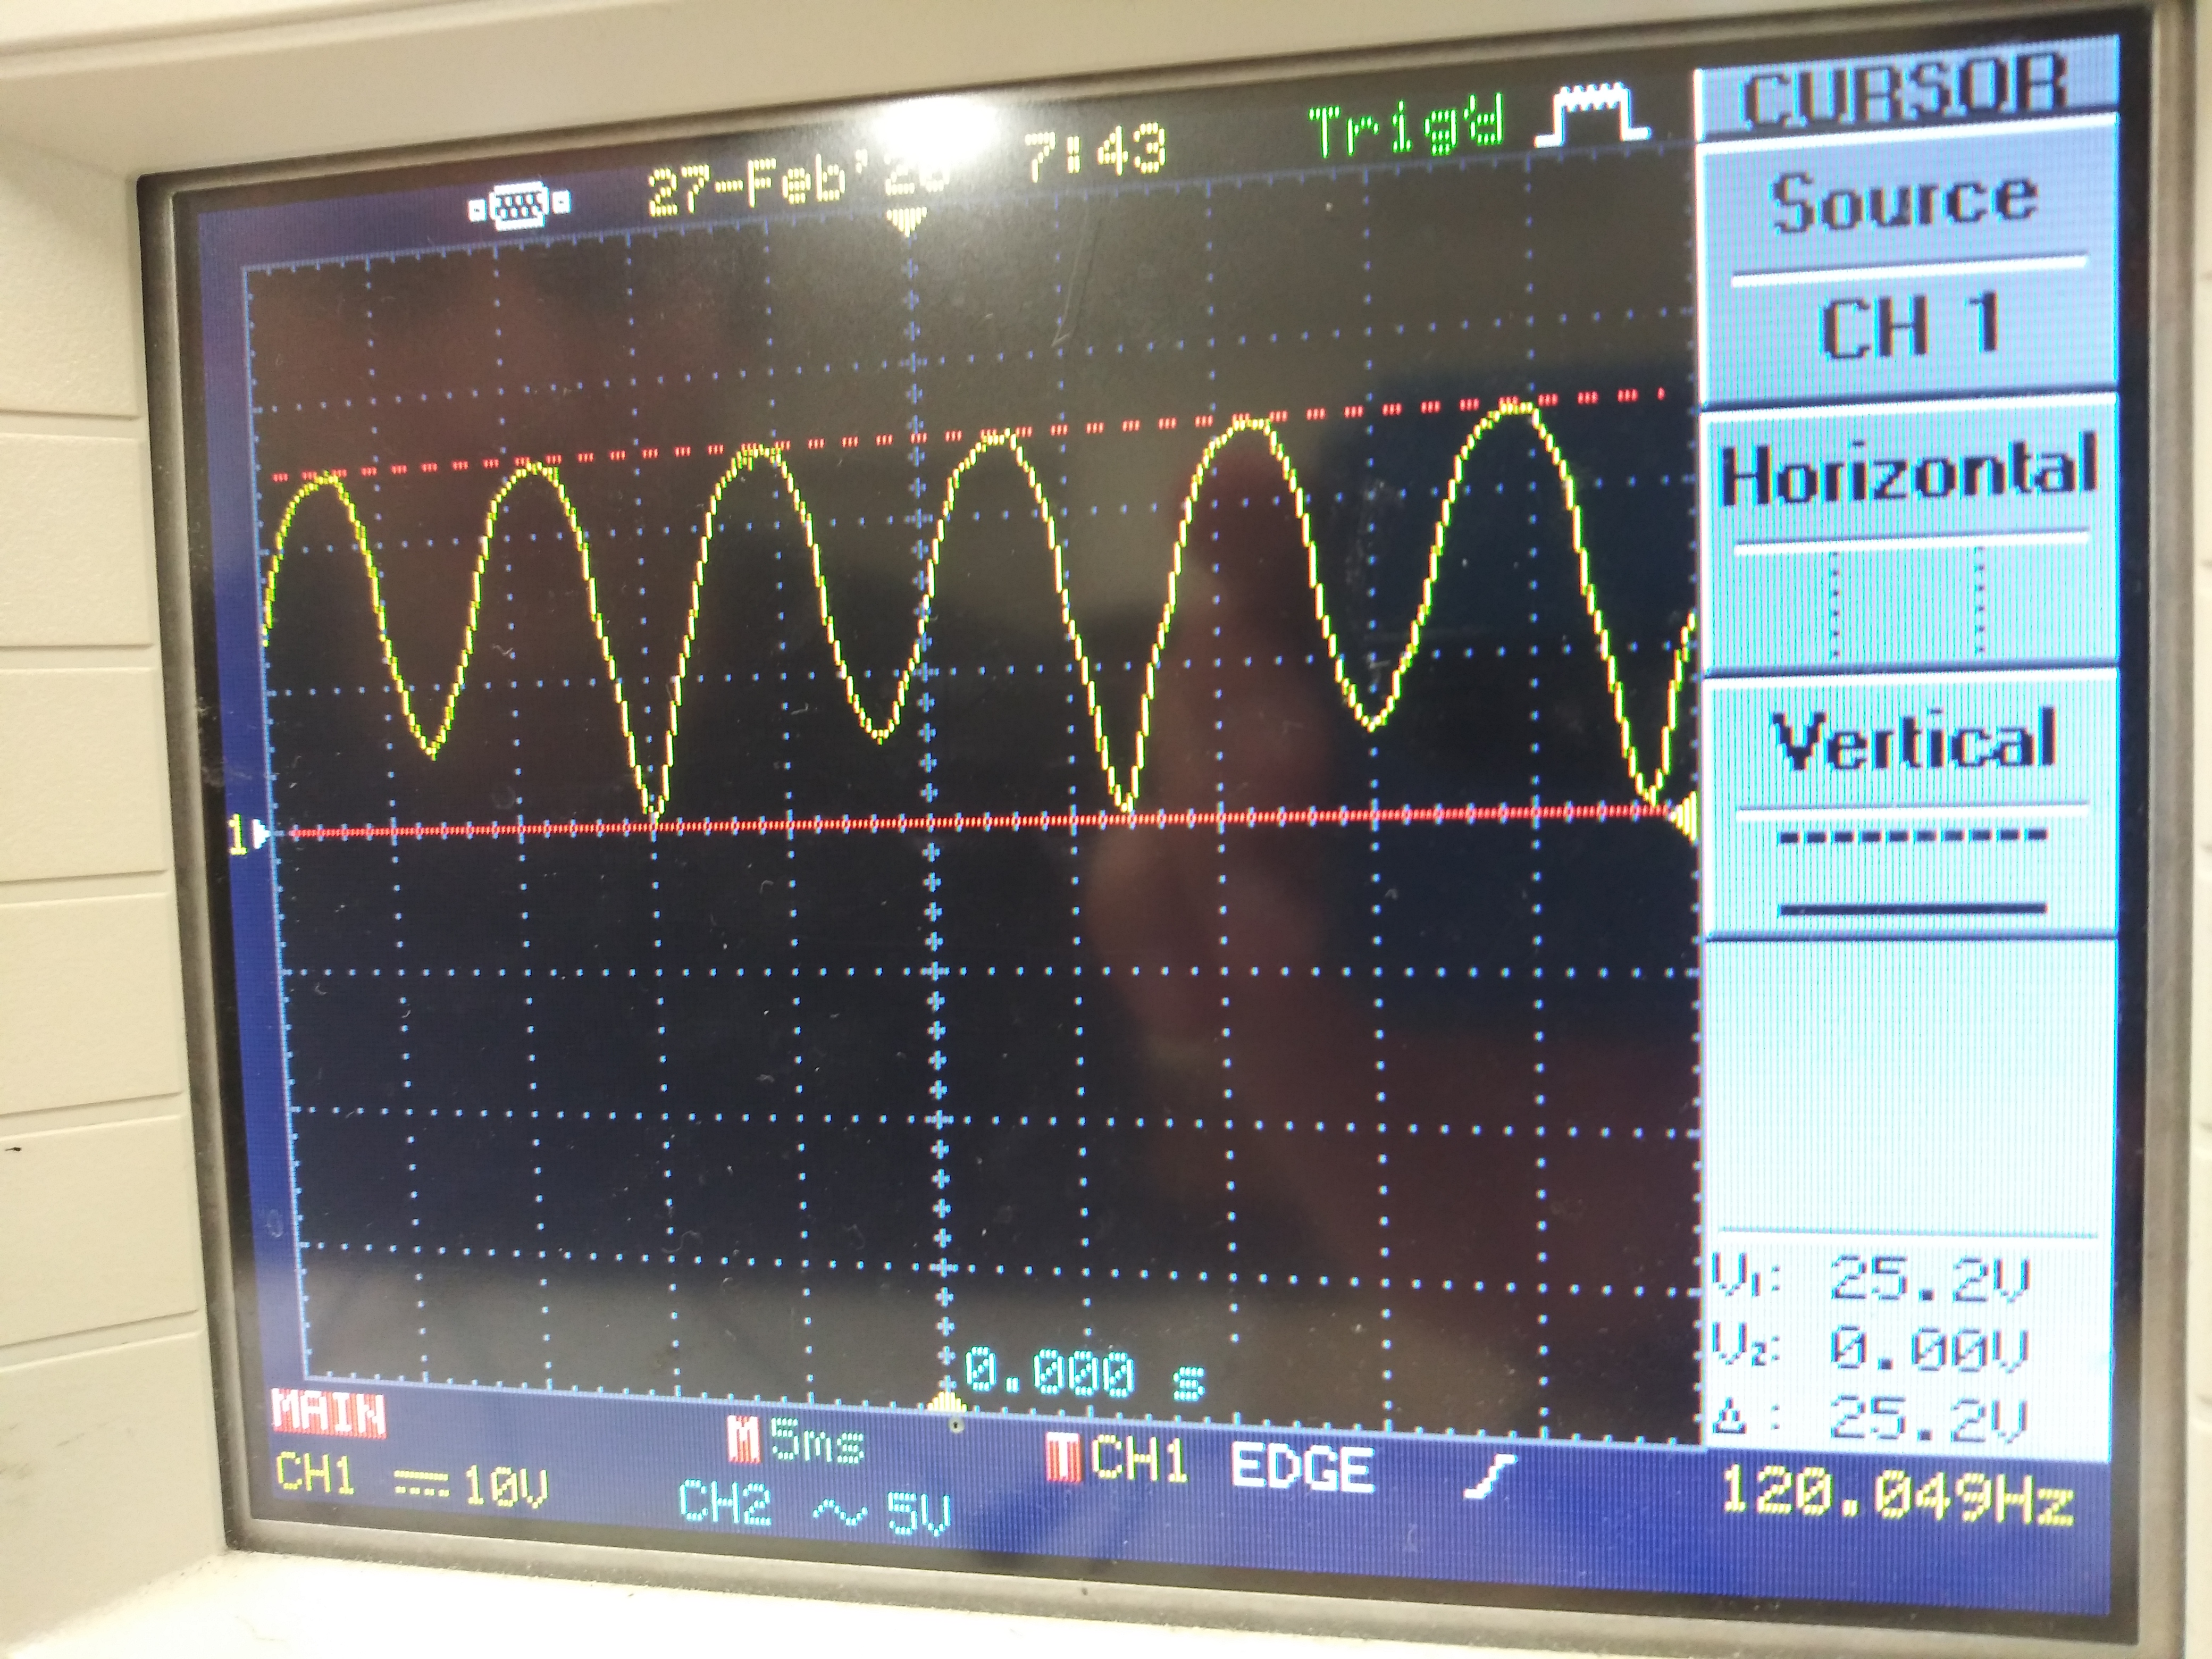
\includegraphics[width=\textwidth]{Images/20200227_181858.jpg}
    \caption{Oscilloscope output from full-wave bridge rectifier.}
    \label{fig7}
\end{figure}

There is a small problem with the output of this circuit, and
that is that half of the periods do not touch \SI{0}{V}. This
is likely due to a problem with the transformer, but if this
flaw is ignored, then the output looks exactly like the simulated
output in Figure 6; that is, the signal bounces up and down
without going into the negative voltage region.

As it can be seen in the measurement of the oscilloscope output,
the measured frequency of the rectifier is \SI{120.049}{\hertz},
which corroborates with the calculated and expected
\SI{120}{\hertz}. The peak voltage of this circuit is
\SI{25.2}{V}, which is close to the expected \SI{24.8025}{V}
measured in Figure 6. In this case, the peak voltage is the
same as the peak--peak voltage because the signal does not
dip down below \SI{0}{V}.

For comparison's sake, the oscilloscope output from Figure 2
of the secondary windings are compiled here. The measured
frequency is \SI{59.9835}{\hertz}, close to the expected
\SI{60}{\hertz}. the peak--peak voltage is \SI{53.2}{V},
which makes the peak voltage
\( \SI{53.2}{V} / 2 = \SI{26.6}{V} \).

\section{Adding a Capacitor} To smooth out the waveform to
something resembling DC voltage, it is necessary to add
a capacitor in parallel. Doing so will make a flatter curve.
Below is the output of the voltage across a \SI{100}{\ohm}
load resistor with a \SI{2200}{\micro\farad} capacitor in
parallel with it.

\begin{figure}[h]
    \centering
    \includegraphics[width=\textwidth]{Images/RectCapacitor.jpg}
    \caption{Output with capacitor in parallel.}
    \label{fig8}
\end{figure}

As it is evident, the signal is not exactly a straight line.
The highest voltage is \SI{24.5654}{V} and the lowest voltage is
\SI{23.9123}{V}, which makes the ripple voltage
\(V_\text{ripple} = \SI{24.5654}{V} - \SI{23.9123}{V}
= \SI{653.1}{\milli\volt}\). The ripple voltage is given by
\begin{equation*}
    V_\text{rip} = \frac{I}{2fC} = \frac{V_p}{2fRC}
\end{equation*} where \(I\) is the current going through
the load resistance, \(f\) is the frequency of the input voltage,
\(C\) is the capacitance of the capacitor in parallel with the
load resistance, \(V_p\) is the peak input voltage, and
\(R\) is the resistance of the load resistor. Inputting the known
values for the right side of the equation, we have the following:
\begin{equation*}
    V_\text{rip} = \frac{V_p}{2fRC}
    = \frac{\SI{26.2}{V}}{2\cdot \SI{100}{\ohm} \cdot \SI{2200}{\milli F}}
    \approx \SI{992.4}{\milli V}
\end{equation*} There is a \SI{339.3}{mV} difference between
the calculated value and the measured value, which is a 
34.2\% error.

\section{Adding a Capacitor (Physical)}

\end{document}
